\documentclass[11pt,fleqn]{article}
%\usepackage{CJK}
\usepackage{latexsym}
\usepackage{color}
\usepackage{graphicx, float}\usepackage{graphicx}
\usepackage{algorithmic}
\usepackage{algorithm}
%\usepackage{algpseudocode}
%\usepackage[colorlinks]{hyperref}
\usepackage[toc,page]{appendix}
\usepackage{bm}
\setlength{\oddsidemargin}{-0.0in}
\setlength{\evensidemargin}{-0.0in} \setlength{\textwidth}{6.0in}
\setlength{\textheight}{9.0in} \setlength{\topmargin}{-0.2in}
%\usepackage[boxruled]{algorithm2e}

%\setlength{\leftmargin}{0.7in}
\usepackage{amssymb, graphicx, amsmath}  %  fancyheadings,
\usepackage{setspace}
\newcommand\qed{\qquad $\square$}
\newcommand{\nn}{\nonumber}

\usepackage{lipsum}

\usepackage{listings}
\lstset{
  basicstyle=\ttfamily,
  columns=fullflexible,
  frameround=fttt,
  breaklines=true,
  %postbreak=\mbox{\textcolor{red}{$\hookrightarrow$}\space},
}

\definecolor{mGreen}{rgb}{0,0.6,0}
\definecolor{mGray}{rgb}{0.5,0.5,0.5}
\definecolor{mPurple}{rgb}{0.58,0,0.82}
\definecolor{backgroundColour}{rgb}{0.95,0.95,0.92}

\lstdefinestyle{CStyle}{
    backgroundcolor=\color{backgroundColour},   
    commentstyle=\color{mGreen},
    keywordstyle=\color{magenta},
    numberstyle=\tiny\color{mGray},
    stringstyle=\color{mPurple},
    basicstyle=\footnotesize,
    breakatwhitespace=false,         
    breaklines=true,                 
    captionpos=b,                    
    keepspaces=true,                 
    numbers=left,                    
    numbersep=5pt,                  
    showspaces=false,                
    showstringspaces=false,
    showtabs=false,                  
    tabsize=2,
    language=C
}

\def \[{\begin{equation}}
\def \]{\end{equation}}
\def\proof{{\bf Proof:\quad}}
\def \endzm {\quad $\Box$}
\def\dist{\hbox{dist}}

\usepackage{tabularx,booktabs}
\newcolumntype{C}{>{\centering\arraybackslash\hsize=.5\hsize}X} % centered version of "X" type
\setlength{\extrarowheight}{1pt}
\usepackage{caption}% <-- added


\newcommand{\R}{\mathbb{R}}
%\newtheorem{yinli}{����}[section]
\newcommand{\D}{\displaystyle}
\newcommand{\T}{\textstyle}
\newcommand{\SC}{\scriptstyle}
\newcommand{\FT}{\footnotesize}

\usepackage{hyperref}
\newcommand\fnurl[2]{%
  \href{#2}{#1}\footnote{\url{#2}}%
}


%\newtheorem{theorem}{Theorem}[section]
%\renewcommand{\thetheorem}{\arabic{section}.\arabic{theorem}}
\newtheorem{definition}{Definition}
\renewcommand{\thedefinition}{\arabic{section}.\arabic{definition}}
\newtheorem{lemma}{Lemma}[section]
\renewcommand{\thelemma}{\arabic{section}.\arabic{lemma}}
\newtheorem{remark}{Remark}
\renewcommand{\theremark}{\arabic{section}.\arabic{remark}}
\newtheorem{proposition}{Proposition}[section]
\renewcommand{\theproposition}{\arabic{section}.\arabic{proposition}}
\newtheorem{corollary}{Corollary }[section]
\renewcommand{\thecorollary}{\arabic{section}.\arabic{corollary}}
\renewcommand{\theequation}{\arabic{section}.\arabic{equation}}
\renewcommand{\baselinestretch}{1.35}
\newtheorem{exam}{Example}[section]
\renewcommand{\theexam}{\arabic{section}.\arabic{exam}}
\newtheorem{theo}{Theorem}[section]
\renewcommand{\thetheo}{\arabic{section}.\arabic{theo}}

% Define a \HEADER{Title} ... \ENDHEADER block
\makeatletter
\newcommand{\HEADER}[1]{\ALC@it\underline{\textsc{#1}}\begin{ALC@g}}
\newcommand{\ENDHEADER}{\end{ALC@g}}
\makeatother

\newcommand{\argmin}{\operatornamewithlimits{argmin}}
\newcommand{\argmax}{\operatornamewithlimits{argmax}}

\usepackage{url} % to make url in bibtex shows up

\usepackage{enumitem}
\newenvironment{QandA}{\begin{enumerate}\bfseries}
                      {\end{enumerate}}
\newenvironment{answered}{\par\normalfont}{}

\begin{document}
%\begin{CJK*}{GBK}{song}

\begin{center}

{\LARGE \bf CloudSuite Investigation Phase I Report}\\

\vskip 25pt
 {Zeyuan Hu, iamzeyuanhu@utexas.edu }\\
\vskip 5pt
{\small EID:zh4378 Spring 2018 }

\end{center}

\begin{spacing}{1.5}
\begin{abstract}

\noindent In this writeup, we investigate the working behavior of the CloudSuite benchmark \cite{Ferdman:2012:CCS:2248487.2150982}.
\end{abstract}

\section{Introduction}

We use a machine that has 4 Intel(R) Core(TM) i5-6200U CPU @ 2.30GHz processors and 4GB of memory. The machine runs 
Ubuntu 16.04.3 (kernel version 4.4.0-116-generic). CloudSuite benchmark contains a collection of benchmarks for different
\fnurl{real-life scenarios}{http://cloudsuite.ch//pages/download/}) (e.g., Data Analytics, Media Streaming, etc). We focus
on the benchmark for \fnurl{web serving}{http://cloudsuite.ch//pages/benchmarks/webserving/}.


The benchmark contains four components: \lstinline|web_server|(represents the web server),
\lstinline|memcached_server|(represents the memcached server), \lstinline|db_server|(represents the database server, which runs MySQL), and
\lstinline|faban_client|(represents the faban client). We run all four components on the same host.

\section{Benchmark Setup}

We follow the instruction on the \fnurl{web serving page}{http://cloudsuite.ch//pages/benchmarks/webserving/}. We first start the database server
by first downloading the corresponding dockerfile:

\begin{lstlisting}
docker pull cloudsuite/web-serving:db_server
\end{lstlisting}

Then, we start the database server:

\begin{lstlisting}
docker run --security-opt seccomp:unconfined -dt --net=host --name=mysql_server cloudsuite/web-serving:db_server localhost
\end{lstlisting}

Similarly, we download the memcached server and the web server dockerfiles, and start them up:

\begin{lstlisting}
docker pull cloudsuite/web-serving:memcached_server
docker pull cloudsuite/web-serving:web_server

docker run --security-opt seccomp:unconfined -dt --net=host --name=memcache_server cloudsuite/web-serving:memcached_server
docker run --cap-add SYS_PTRACE --security-opt seccomp:unconfined -dt --net=host --name=web_server cloudsuite/web-serving:web_server /etc/bootstrap.sh
\end{lstlisting}

\lstinline|--cap-add SYS_PTRACE| allows us to invoke \texttt{strace} \fnurl{command}{http://www.skrenta.com/rt/man/strace.1.html} inside the docker. Finally, we download the faban client and run the benchmark

\begin{lstlisting}
docker pull cloudsuite/web-serving:faban_client
docker run --security-opt seccomp:unconfined --net=host --name=faban_client cloudsuite/web-serving:faban_client localhost
\end{lstlisting}

\section{Experiments}

We focus on the \lstinline|web_server| component in the experiment. The \lstinline|web_server| consists of \fnurl{elgg framework}{https://elgg.org/} (a web development framework), \fnurl{Nginx}{http://nginx.org/}(a web server), and \fnurl{PHP-FPM}{https://php-fpm.org/}(a PHP implementation
of a variant of Common Gateway Interface(CGI)). The goal of our experiment is to understand the communication behavior between PHP-FPM and Nginx by
answer the following questions.

\begin{QandA}
\item When running the benchmark, Nginx will create worker processes. How many worker processes will Nginx create during the benchmark?
\begin{answered}
We login to the \lstinline|web_server| docker by executing \lstinline|sudo docker exec -it \web_server bash| and then we issue \lstinline|ps -fax|
and the output is shown in Figure \ref{ps-fax}. As one can see, the Nginx creates four worker processes.

\begin{figure}
\centering
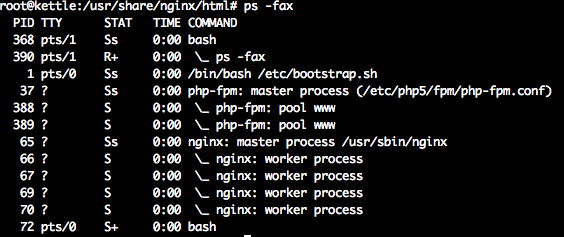
\includegraphics[scale=0.8]{ps-fax.png} 
\caption{Inside \texttt{web\_server} docker}
\label{ps-fax}
\end{figure}

\end{answered}

\item Does Nginx create worker process on demand or create all of them before the test is running? 
\begin{answered}
Nginx creates all the worker processes before the test is running. We can run \lstinline|strace -p 65| and \texttt{65} is the PID
of the Nginx master process and we see the following

\begin{lstlisting}
root@kettle:/usr/share/nginx/html# strace -p 65
Process 65 attached
rt_sigsuspend([]
\end{lstlisting}

Master process is being suspended and wait for a signal to invoke signal handler or terminate process. In other words, even
the test is running, the master process already finishes its job (i.e., spawning the worker processes) and thus, being suspended.

\end{answered}

\item Will PHP-FPM create worker processes?
\begin{answered}
Yes. If we use \lstinline|strace -f -q -s 100 -o app.trc -ff -p 37| \footnote{\lstinline|-s 100| means the max string length for each line in \texttt{app.trc} is 100. Use larger value if you don't want the line get truncated (e.g., \texttt{2000}).}, which is to trace system calls and signals and we
see that

\begin{lstlisting}
root@kettle:/usr/share/nginx/html# strace -f -s 100 -o app.trc -ff -p 37
Process 37 attached
Process 2007 attached
Process 2008 attached
Process 2009 attached
Process 2010 attached
Process 2011 attached
Process 2012 attached
Process 2013 attached
Process 2014 attached
Process 2015 attached
Process 2016 attached
Process 2017 attached
^CProcess 37 detached
Process 2017 detached
Process 2016 detached
\end{lstlisting}

and if we open the trace file (\texttt{app.trc.37}) of PHP-FPM master process (with PID 37), we can see the following

\begin{lstlisting}
epoll_wait(9, 125b530, 1, 973)          = -1 EINTR (Interrupted system call)
--- SIGCHLD {si_signo=SIGCHLD, si_code=CLD_DUMPED, si_pid=2000, si_status=SIGBUS, si_utime=1, si_stime=2} ---
write(7, "C", 1)                        = 1
rt_sigreturn()                          = -1 EINTR (Interrupted system call)
epoll_wait(9, {{EPOLLIN, {u32=15543904, u64=15543904}}}, 1, 432) = 1
read(5, "C", 1)                         = 1
wait4(-1, [{WIFSIGNALED(s) && WTERMSIG(s) == SIGBUS && WCOREDUMP(s)}], WNOHANG|WSTOPPED, NULL) = 2000
write(4, "[21-Apr-2018 15:39:51] WARNING: [pool www] child 2000 exited on signal 7 (SIGBUS - core dumped) afte"..., 130) = 130
clone(child_stack=0, flags=CLONE_CHILD_CLEARTID|CLONE_CHILD_SETTID|SIGCHLD, child_tidptr=0x7f75e88eca10) = 2007
write(4, "[21-Apr-2018 15:39:51] NOTICE: [pool www] child 2007 started\n", 61) = 61
wait4(-1, 0x7ffe87eab74c, WNOHANG|WSTOPPED, NULL) = 0
read(5, 0x7ffe87eab83f, 1)              = -1 EAGAIN (Resource temporarily unavailable)
epoll_wait(9, {}, 1, 432)               = 0
epoll_wait(9, 125b530, 1, 1000)         = -1 EINTR (Interrupted system call)
--- SIGCHLD {si_signo=SIGCHLD, si_code=CLD_DUMPED, si_pid=2001, si_status=SIGBUS, si_utime=0, si_stime=0} ---
write(7, "C", 1)                        = 1
rt_sigreturn()                          = -1 EINTR (Interrupted system call)
epoll_wait(9, {{EPOLLIN, {u32=15543904, u64=15543904}}}, 1, 274) = 1
...
\end{lstlisting}

\lstinline|clone| indicates that PHP-FPM master process clones a child process and the master process then 
wait for the child process. \lstinline|epoll_wait| waits for an I/O event on an epoll file descriptor. In this case,
when child exits, the master process will read from file descriptor and record child status.

\end{answered}

\item How does Nginx setup the communication channel with PHP-FPM?
\begin{answered}
We use the strace again \lstinline|strace -f -s 100 -o nginx.trc -p 69| and we do \lstinline|grep socket nginx.trc| and \lstinline|grep connect nginx.trc| and we see the following

\begin{lstlisting}
root@kettle:/usr/share/nginx/html# grep socket nginx.trc
69    socket(PF_LOCAL, SOCK_STREAM, 0)  = 15
69    socket(PF_LOCAL, SOCK_STREAM, 0)  = 15
69    socket(PF_LOCAL, SOCK_STREAM, 0)  = 15
69    socket(PF_LOCAL, SOCK_STREAM, 0)  = 15
69    socket(PF_LOCAL, SOCK_STREAM, 0)  = 15
69    socket(PF_LOCAL, SOCK_STREAM, 0)  = 15

root@kettle:/usr/share/nginx/html# grep connect nginx.trc
69    connect(15, {sa_family=AF_LOCAL, sun_path="/var/run/php5-fpm.sock"}, 110) = 0
69    connect(15, {sa_family=AF_LOCAL, sun_path="/var/run/php5-fpm.sock"}, 110) = 0
69    connect(15, {sa_family=AF_LOCAL, sun_path="/var/run/php5-fpm.sock"}, 110) = 0
69    connect(15, {sa_family=AF_LOCAL, sun_path="/var/run/php5-fpm.sock"}, 110) = 0
69    connect(15, {sa_family=AF_LOCAL, sun_path="/var/run/php5-fpm.sock"}, 110) = 0
69    connect(15, {sa_family=AF_LOCAL, sun_path="/var/run/php5-fpm.sock"}, 110) = 0
\end{lstlisting}

Thus, we can say that Nginx communicates with PHP-FPM using sockets.

\end{answered}

\item Does the channel setup when a new worker process is created? Or when the worker process wants to talk to PHP-FPM? 
\begin{answered}
The channel sets up when the worker process want to talk to PHP-FPM. For each worker process, we issue
\lstinline|strace -f -s 100 -o nginx.trc -p <worker_pid>| and we can see some worker performs \lstinline|epoll_wait|
all the time while other workers are talking with PHP-FPM:

\begin{lstlisting}
root@kettle:/usr/share/nginx/html# strace -f -s 100 -p 66
Process 66 attached
epoll_wait(13, {}, 512, 500)            = 0
epoll_wait(13, {}, 512, 500)            = 0
epoll_wait(13, {}, 512, 500)            = 0
epoll_wait(13, {}, 512, 500)            = 0
epoll_wait(13, {}, 512, 500)            = 0

root@kettle:/usr/share/nginx/html# strace -f -s 100 -p 70
Process 70 attached
epoll_wait(19, {{EPOLLIN, {u32=2707665296, u64=140164670402960}}}, 512, -1) = 1
accept4(10, {sa_family=AF_INET, sin_port=htons(34074), sin_addr=inet_addr("127.0.0.1")}, [16], SOCK_NONBLOCK) = 12
epoll_ctl(19, EPOLL_CTL_ADD, 12, {EPOLLIN|EPOLLET, {u32=2707665872, u64=140164670403536}}) = 0
epoll_wait(19, {{EPOLLIN, {u32=2707665872, u64=140164670403536}}}, 512, 60000) = 1
recvfrom(12, "HEAD / HTTP/1.1\r\nHost: localhost:8080\r\nUser-Agent: curl/7.47.0\r\nAccept: */*\r\n\r\n", 1024, 0, NULL, NULL) = 79
stat("/usr/share/nginx/html/elgg/", {st_mode=S_IFDIR|0755, st_size=4096, ...}) = 0
stat("/usr/share/nginx/html/elgg/", {st_mode=S_IFDIR|0755, st_size=4096, ...}) = 0
stat("/usr/share/nginx/html/elgg/index.php", {st_mode=S_IFREG|0664, st_size=516, ...}) = 0
epoll_ctl(19, EPOLL_CTL_MOD, 12, {EPOLLIN|EPOLLOUT|EPOLLET, {u32=2707665872, u64=140164670403536}}) = 0
getsockname(12, {sa_family=AF_INET, sin_port=htons(8080), sin_addr=inet_addr("127.0.0.1")}, [16]) = 0
socket(PF_LOCAL, SOCK_STREAM, 0)        = 14
ioctl(14, FIONBIO, [1])                 = 0
...
\end{lstlisting}

Thus, the connection is established when the worker process wants to talk to PHP-FPM.

% Nginx + PHP-FPM: https://www.nginx.com/resources/wiki/start/topics/examples/phpfcgi/

\end{answered}
\end{QandA}

\end{spacing}

\bibliographystyle{ieeetr}
\bibliography{report}


\end{document}

